\documentclass{aip-cp}

\usepackage[numbers]{natbib}
\usepackage{rotating}
\usepackage{graphicx}
\usepackage[dvipsnames]{xcolor}
\usepackage{url}

\newif\iffinal
% Un-comment this line to see proposal without comments
%\finaltrue

\iffinal
    \newcommand\ian[1]{}
    \newcommand\ben[1]{}
    \newcommand\ryan[1]{}
    \newcommand\kyle[1]{}
\else
    \newcommand\ian[1]{{\color{red}[Ian: #1]}}
    \newcommand\ben[1]{{\color{blue}[Ben: #1]}}
    \newcommand\ryan[1]{{\color{green}[Ryan: #1]}}
    \newcommand\kyle[1]{{\color{purple}[Kyle: #1]}}
\fi

\newcommand\code[1]{{\tt \footnotesize #1}}
\newcommand\bluecode[1]{\code{#1}}
\newcommand\darkcode[1]{\code{#1}}
%\newcommand\bluecode[1]{{\color{blue}\code{\textbf{#1}}}}
%\newcommand\darkcode[1]{\code{\textbf{#1}}}

% Document starts
\begin{document}

% Title portion
\title{Data Automation at Light Sources}

\author[aff1]{Ben Blaiszik}
\author[aff1]{Kyle Chard}
\author[aff1]{Ryan Chard}
\author[aff1,aff2]{Ian Foster\corref{cor1}}
\author[aff1]{Logan Ward}

\affil[aff1]{Data Science and Learning Division, Argonne National Laboratory, Argonne IL 60439, USA.}
\affil[aff2]{Department of Computer Science, University of Chicago, Chicago IL 60637, USA.}
%\affil[aff3]{You would list an author's second affiliation here.}
\corresp[cor1]{Corresponding author: foster@anl.gov}
%\authornote[note1]{This is an example of first authornote.}
%\authornote[note2]{This is an example of second authornote.}

\maketitle


\begin{abstract}
%The AIP Proceedings article template has many predefined paragraph styles for you to use/apply as you write your paper. To format your abstract, use the \LaTeX template style: {\itshape Abstract.} Each paper must include an abstract. Begin the abstract with the word ``Abstract'' followed by a period in bold font, and then continue with a normal 9 point font.
Rapidly growing data volumes at light sources demand increasingly automated data collection, 
distribution, and analysis processes, in order to enable new scientific discoveries while not 
overwhelming finite human capabilities. I present here the case for automating and outsourcing 
light source science using cloud-hosted data automation and enrichment services, institutional 
computing resources, and high- performance computing facilities to provide cost-effective, scalable, 
and reliable implementations of such processes. I discuss three specific services that accomplish 
these goals for data distribution, automation, and transformation. In the first, such services are 
combined with cloud-hosted data indexing and institutional storage to create a 
collaborative data publication, indexing, and discovery service, the Materials Data Facility (MDF), 
built to support a host of informatics applications in materials science. In the second,  
Globus cloud-hosted data automation services are used to implement data capture, distribution, and 
analysis workflows for Advanced Photon Source and Advanced Light Source beamlines, leveraging 
institutional storage and computing. The third integrates 
components of the previous two projects with machine learning capabilities provided by the Data and 
Learning Hub for science (DLHub) to enable on-demand access to machine learning models from light 
source data capture and analysis workflows, and provides simplified interfaces to train new models 
on data from sources such as MDF on leadership scale computing resources. I draw conclusions about 
best practices for building next-generation data automation systems for future light sources.
\ryan{Map this to the new structure.}
\end{abstract}


\section{INTRODUCTION}

%\ryan{Proposed new structure to follow the talk: Introduction, history/background, automation and 
%outsourcing (high level motivation), acquisition and distribution (dmagic/petrel), publication and 
%discovery (mdf/search), automation (automate, TAP), transformation and analysis (dlhub).}

Light source scientists are facing a data crisis as the rate at which new instruments generate data 
volumes is rapidly exceeding Moore's Law~\cite{toby2015practices}. Growing data 
volumes present new challenges as they overwhelm finite human capabilities, requiring new 
machine-based solutions to automate and outsource the acquisition, analysis, and 
distribution of 
light science data. Neither humans or computers can cope using current methods. Existing 
techniques to design experiments, manage and analyze data, and create and 
deliver software will not suffice for next generation data rates. However, these 
challenges also present new opportunities and offer the potential to create the new automation 
systems and enrichment services necessary to utilize instrument advancements. New 
approaches are required to unburden scientists from time consuming data munging, management, 
and dissemination practices, including reliably indexing and cataloging, pipelining, and 
transforming results.

Fourth-generation light sources such as the Advanced Photon Source Upgrade (APS-U)~\cite{APSU} will offer exciting new
scientific capabilities to the thousands of scientists who use their many beamlines annually.
They also pose major data and computation challenges, for at least four reasons.
First, they will generate massive data. 
For example, x-ray photon correlation spectroscopy can already generate 2MB images at 3,000 Hz,
for a data rate of 6 GB/s, comparable to that of the Large Hadron Collider~\cite{lhcrate}.
With APS-U, this data rate is expected to increase by 2--3 orders of magnitude.
Second, experiments will increasingly generate complex multi-modal data that needs advanced computing
for interpretation, such as ptychography combined with 
elemental mapping and visual images as a function of reaction conditions.
Third, it will become increasingly feasible to use advanced theory and modeling to fit and co-optimize 
model and experiment. 
% to increase experiment efficiency and maximize limited experiment and simulation resources.
Fourth, as synchrotron light sources mature as instruments, they increasingly serve more and 
different users,
many with limited or no experience with light sources. 
Automation is important for such users~\cite{hiraki2008high,toby2009management}.

For light science to exploit these advancements the tools and services must transition from an
artisanal/cottage industry to one that builds on 
automated solutions that are integrated into daily operation of a 
beamline. Tools to automatically capture, apply advanced analyses, and autonomically drive 
experiments are necessary, such as those we have previously explored~\cite{wozniak2015big}. In 
addition, once data are acquired, scientists must outsource their ongoing management and 
distribution through dedicated, community-oriented storage hubs that make discoverable and 
accessible the results of experiments. Storage catalogs, such as the Materials Data 
Facility~\cite{MDF2016}, provide rich environments to foster collaboration and increase the value 
of datasets by disseminating results and in turn, accelerating scientific discovery. Similarly, 
nexuses for applying transformations and analyses provide platforms that federate access to cutting 
edge analyses, optimized high performance modalities, and remove barriers of entry to leadership 
computing facilities.

% RC: not sure what this means.
% Onsite not offsite.

Here we describe our efforts to outsource and automate
data distribution, management, and transformation. We
describe how each enables light source scientists to 
outsource tasks crucial for their science.
% We discuss areas in which we are working to reduce the burden of scientists by 
%developing the tools and techniques needed to reliably manage data. 
First, we present data acquisition and distribution tools and services, 
describing specifically how the Globus data publication platform can enable scalable and 
secure data distribution using powerful data access and discovery capabilities. 
Second, we outline a new Globus cloud-hosted data automation 
service and describe how it can be used to manage sophisticated data lifecycles. 
%We then present the case for automation and the 
%techniques used to enables its application. 
%We then describe data indexing and search tools, such 
%as the Materials Data Facility, to outsource the management of data once it has been created. 
Finally, we explore the data transformation capabilities 
provided by the Data and Learning Hub for science (DLHub) 
to enable simple, yet scalable, training of machine learning models
and on-demand access to machine learning models from light source data capture
and analysis workflows.



\section{BACKGROUND/HISTORY}

We first experimented with online analysis of APS data in the late 1990s, 
when we coupled 
computing microtomography~\cite{wang1999quasi,wang2001high} and crystallographic~\cite{von2000using}
experiments to remote computers.
In one memorable demonstration in 1998, we piped microtomography data from APS beamline 2-BM to a 
96-node SGI Origin parallel computer 
at Argonne for incremental reconstruction via filtered backprojection as an experiment was 
proceeding,
and then streamed visualization data to the Supercomputing conference (SC'98) in Orlando, Florida, 
for interactive analysis: see Figure~\ref{fig:sc98}. 
As we noted at the time, 
``the data rates and compute power required ... are prodigious, easily reaching one gigabit per 
second and a teraflop per second [respectively]"~\cite{von2000real}---numbers that are dwarfed by 
today's requirements. 
These demands have since increased tremendously, as illustrated by recent work on near-real-time tomography~\cite{Bicer_Europar15,bicer2017real}.
%in which XXX.

\begin{figure}[h]
  \centerline{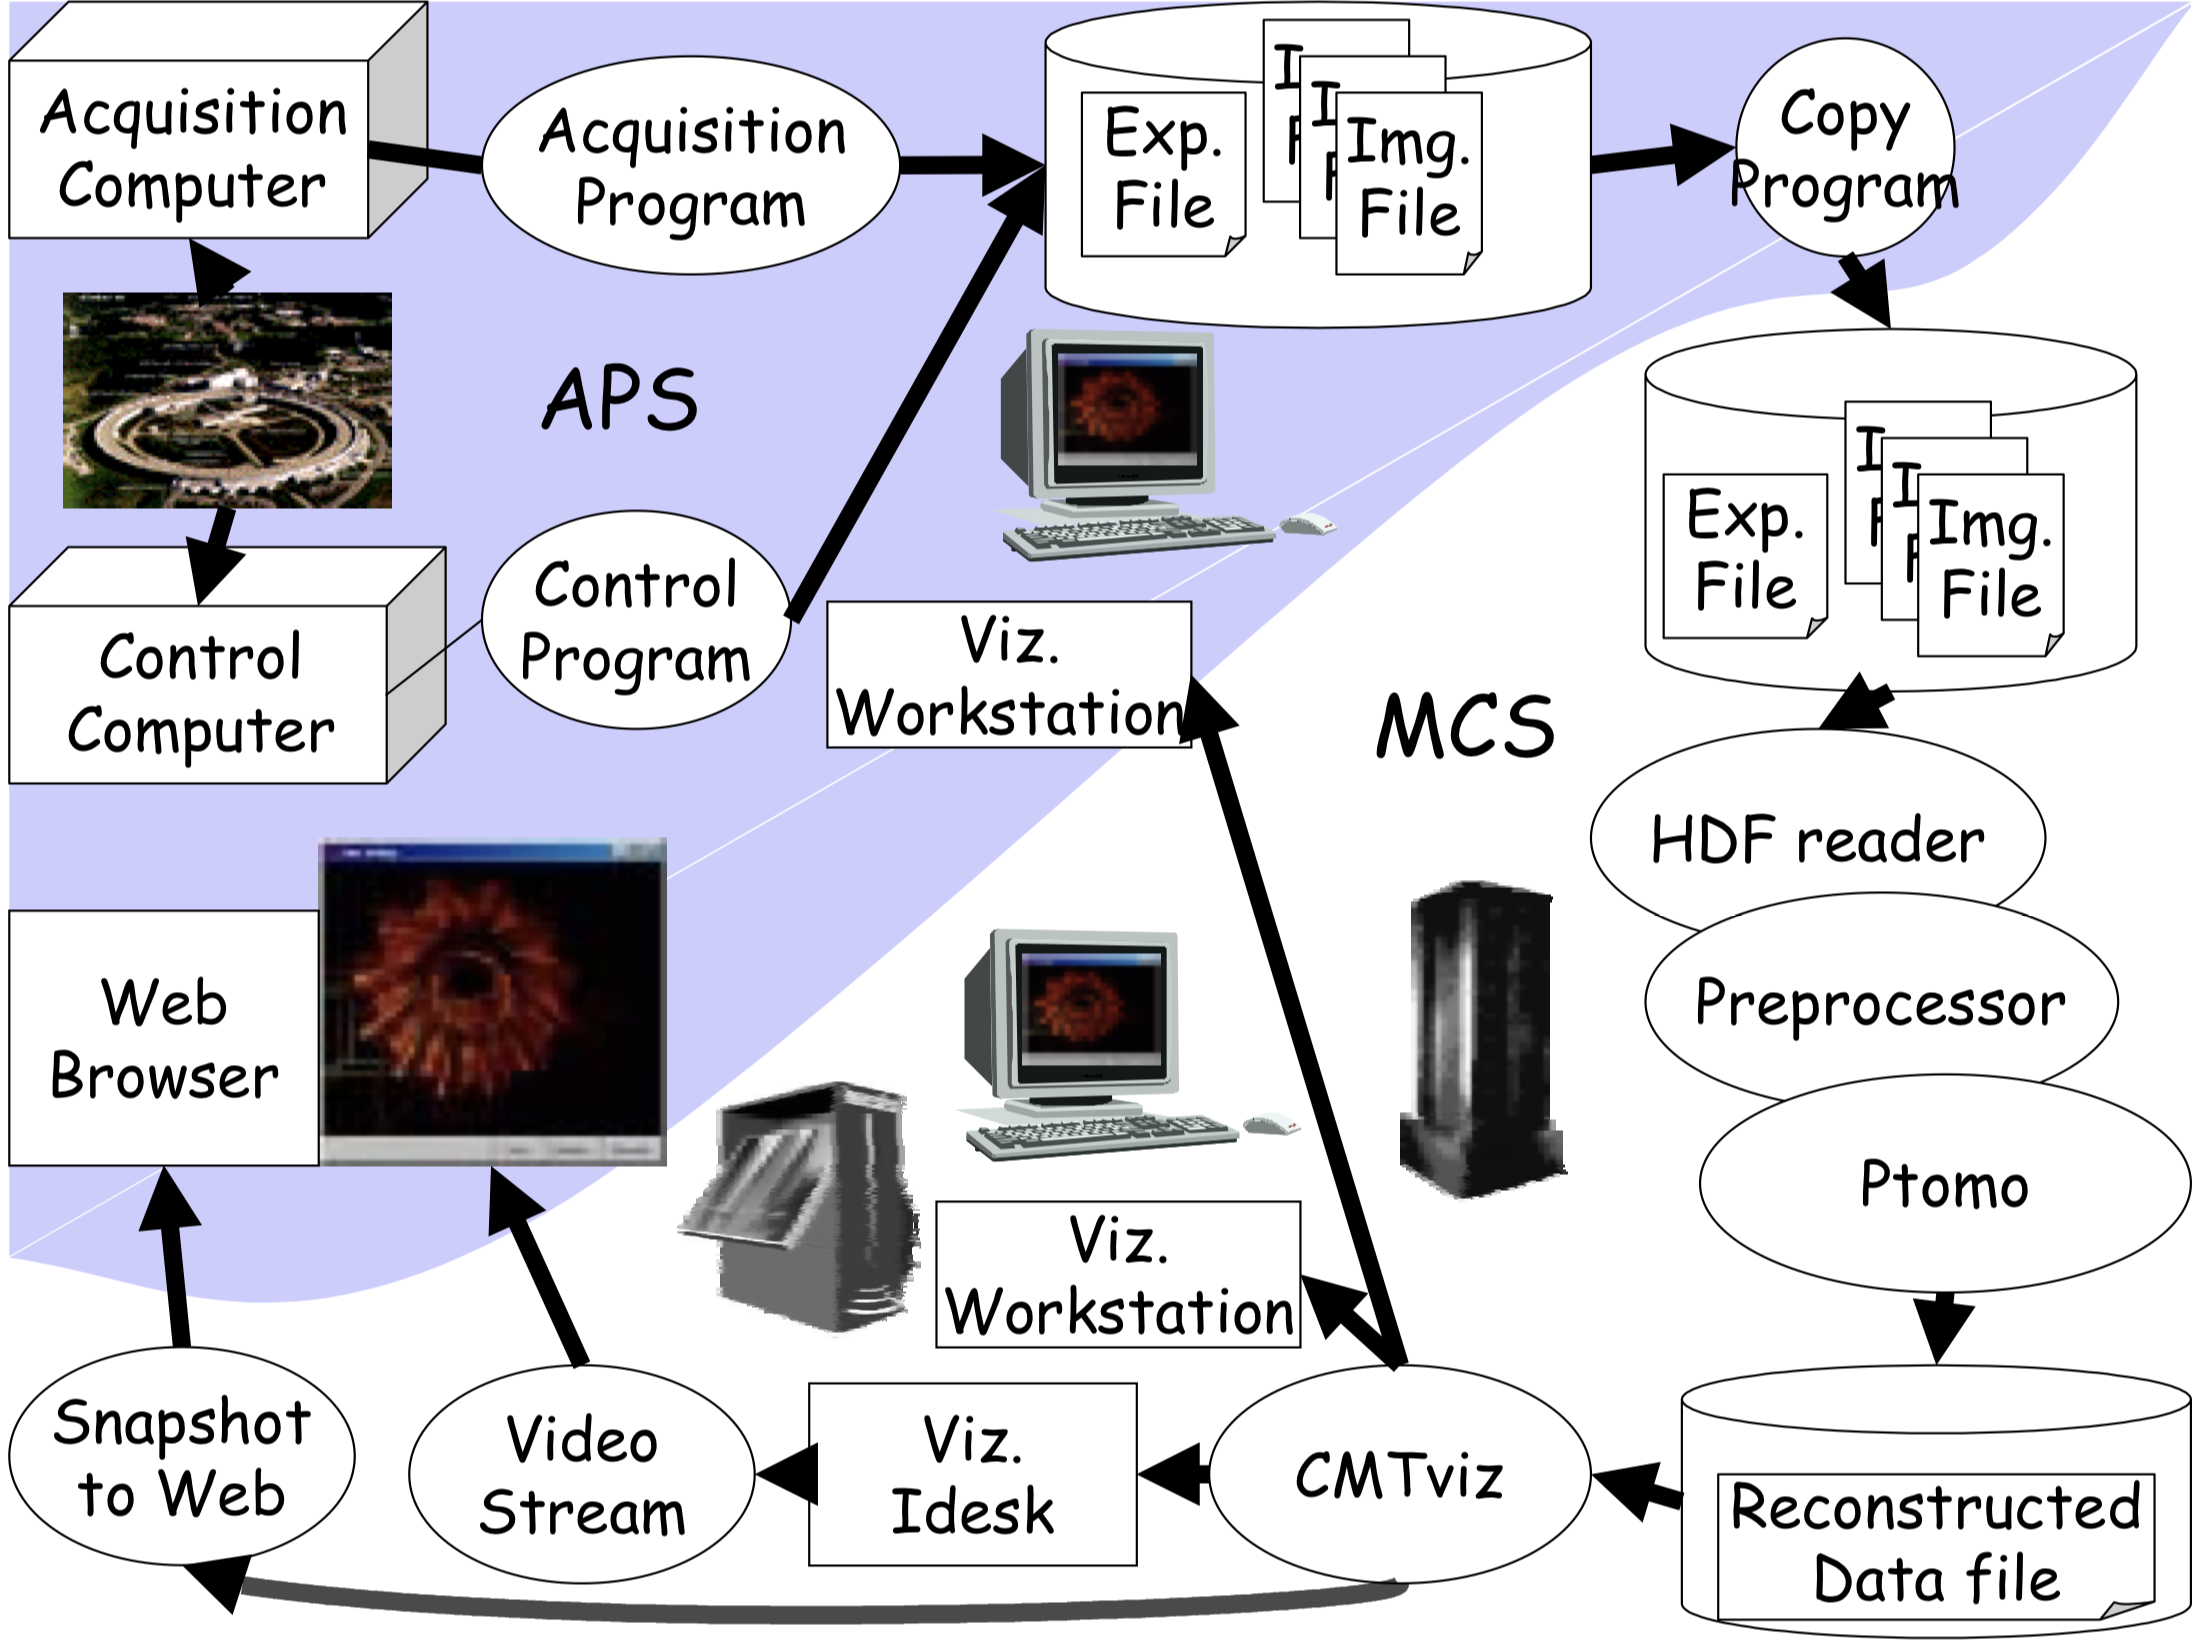
\includegraphics[width=4in]{Figs/APS-Fig.png}}
  \caption{The processing pipeline used in the SC'98 demonstration~\cite{von2000real}. Data 
collected at the APS 
  were passed to a supercomputer in Argonne's Mathematics and Computer Science (MCS) division for
  incremental reconstruction and visualization, and results dispatched as a stereoscopic
  video stream to a remote virtual reality display at APS and in Orlando.\label{fig:sc98}}
\end{figure}

More recently, we have worked to combine experiment and simulations
for diffuse scattering experiments: see Figure~\ref{fig:diffuse}. 
The figure highlights the interactions between experiment, computation, and human expertise
at various timescales. In particular, it shows how simulation and 
experimental workflows can be combined to enable experiment steering and 
rapid validation of experiment results.
On the experiment side, diffuse scattering data are obtained using a beamline.  
High performance computers are used to reconstruct and analyze the data, often in
near real-time to provide rapid feedback to researchers. Here, data is collected
as a sample is rotated 360 degrees in tenth-of-a-degree increments, yielding
3,600 images. Each image comprises 2048$\times$2048 32-
bit pixels, (i.e., 16 MB), a total of 56 GB. Images are
produced at a rate of 10 per second and thus at a peak rate of
160 MB/s. Following the collection of a complete 3,600-image
dataset, which takes about 10 minutes, either a new sample
is inserted or the sample conditions are changed,
and the process is repeated. 


On the simulation side, researchers explore a huge range of synthetic structures
using various high performance software packages, and increasingly machine learning
methods to create simulated output to be compared with, or to help guide, experiments. 
It is important to note, that these experiments and simulations need not be performed
by the same researchers or at the same time. Rather, these simulations are often performed by
collaborations that span institutions and even domains. 
%The resulting datasets derived by both experiments and simulations are further analyzed
%and compared to create a knowledge base that may be used internally, or externally, 
%to further investigate data and guide future exploration.

\begin{figure}[h]
  \centerline{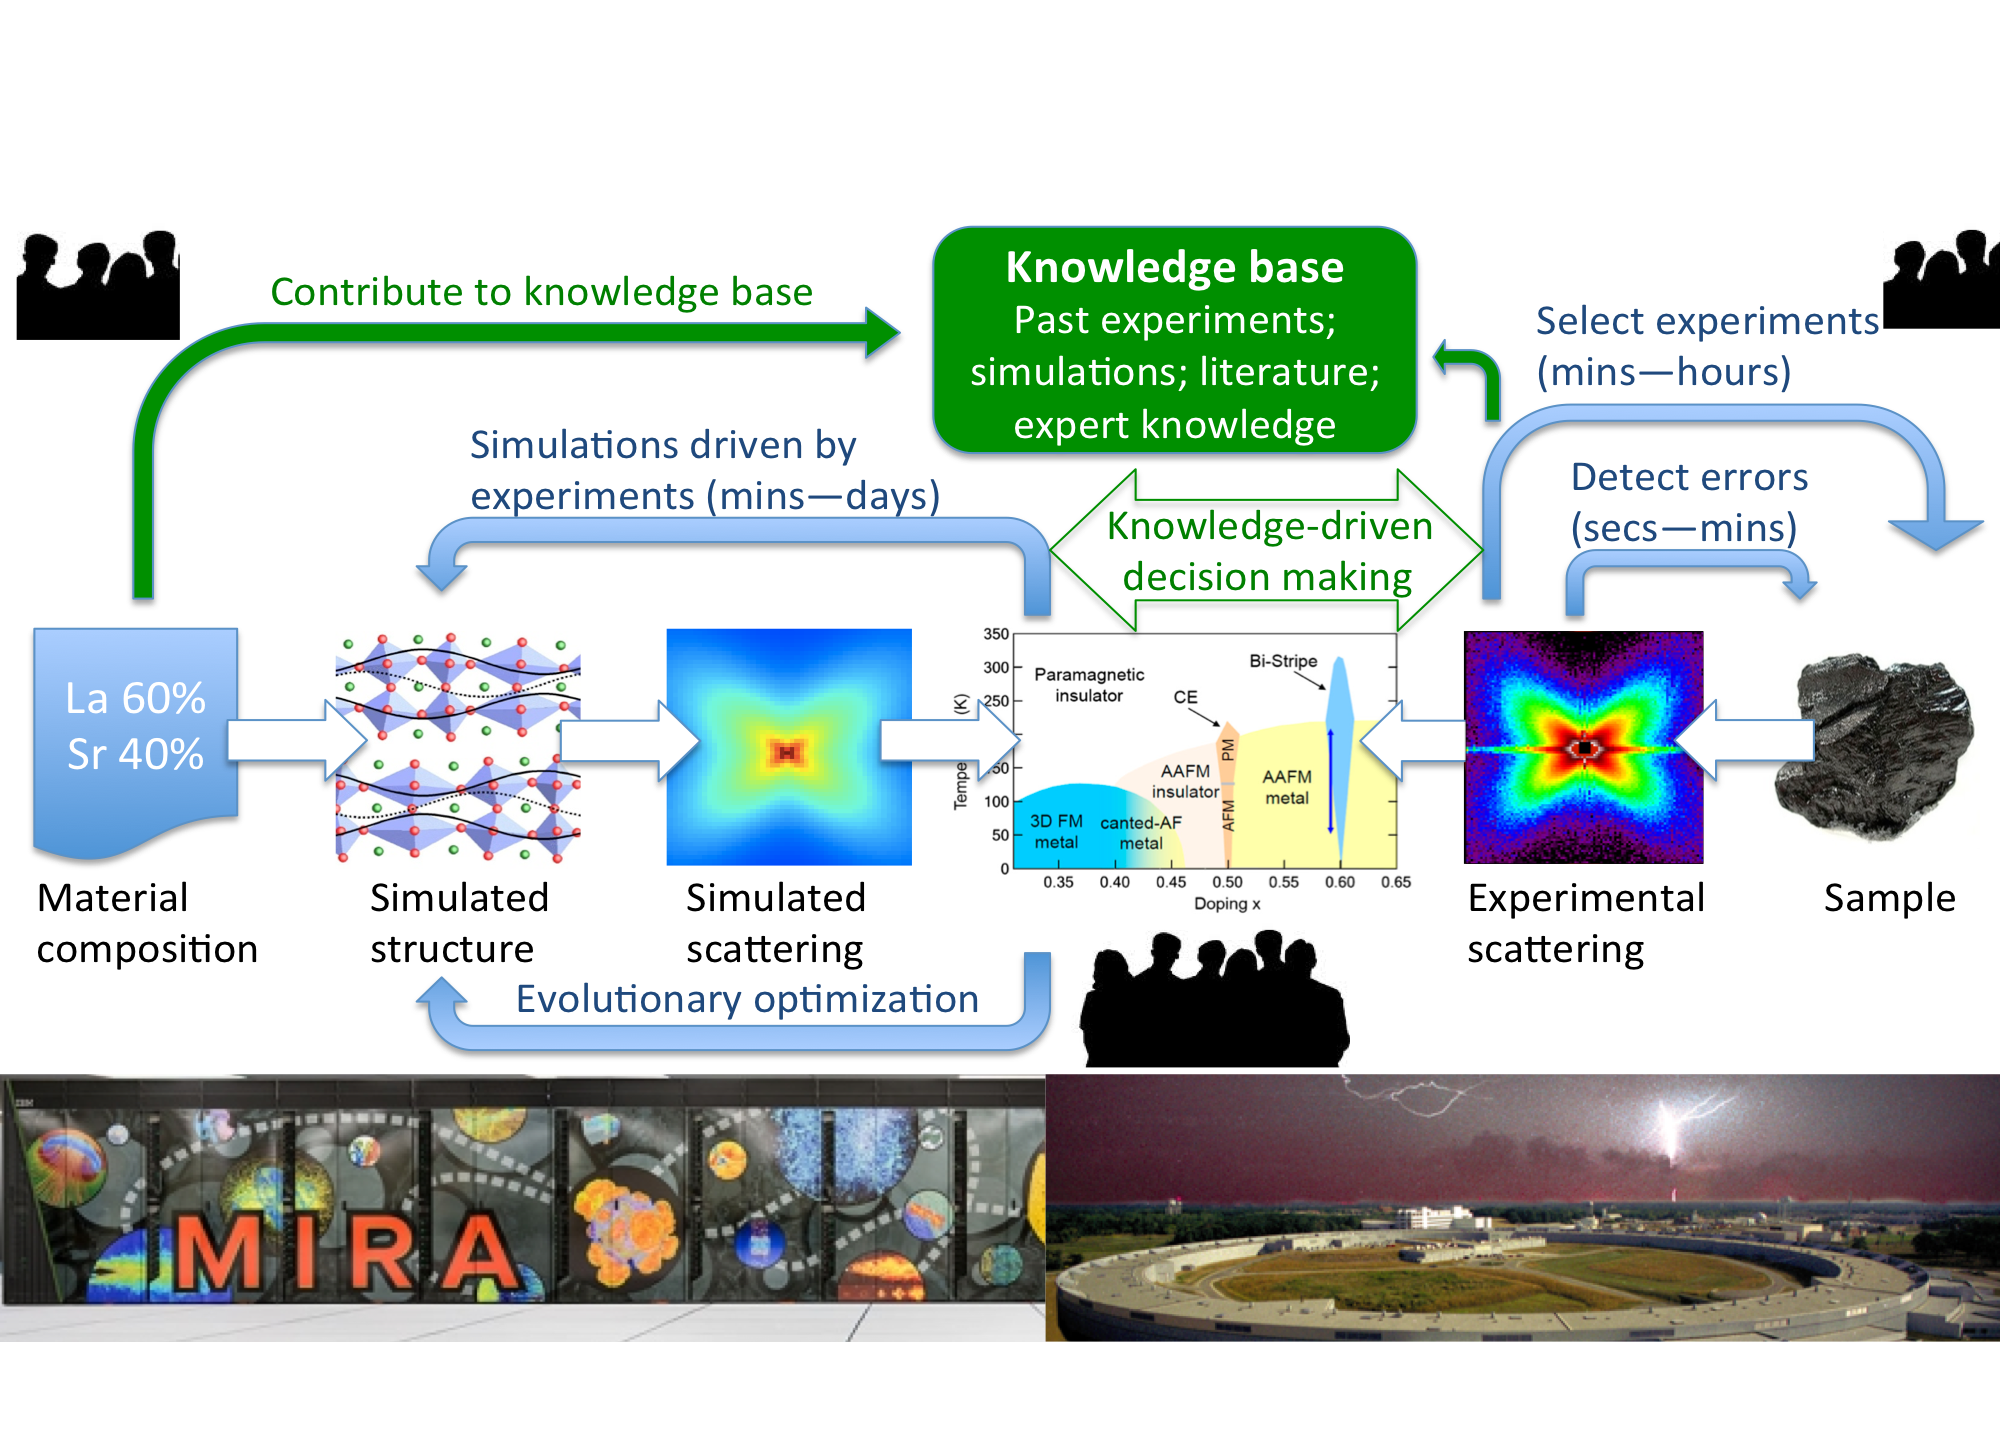
\includegraphics[width=6in,trim=0 2.6in 0 1.5in,clip]{Figs/diffuse.png}}
  \caption{Activities involved in a diffuse scattering experiment. Data is acquired
   via simulation and experimentation, involves data storage in various locations
from beamline computers through to data archives, requires analysis at various scales
and coordination between a diverse group of collaborators. 
  %Acceleration and even automation of these various end-to-end processes, plus the creation of 
powerful knowledge base and simulation capabilities, can create a ``discovery engine'' for materials 
science research. 
  %Note the publication phase by which data is contributed to the growing knowledge base.
\label{fig:diffuse}}
\end{figure}

It is our long history working with light science researchers, experiments,
and simulations that informs our belief that existing methods 
will not meet the requirements of next generation instruments. Indeed, new approaches 
are needed to manage increasing data volumes, design yet more complex
experiments, drive acquisition at unprecedented rates, and apply
and integrate advanced analyses. As we will describe, 
new methods that automate and outsource crucial data management and
manipulation tasks are needed to exploit 
instrument advancements and advance light source science outcomes.



\section{MOTIVATION: AUTOMATION AND OUTSOURCING}

%\ian{Big picture thoughts I guess.}
%
%\ryan{Use this section as motivation for the following ones? I decided to move automate etc. down 
%to its own section and keep this one high level -- like in the talk. Goal of this section is to 
%talk about: automation, human-in-the-loop, outsourcing, and motivate the 3 coming sections.}


As the scale and complexity of light-source science continues to grow, so too
does the burden on researchers to manage an increasingly complex ecosystem of
data, software, and cyberinfrastructure.  Unfortunately, these burdens are
increasingly prohibitive as the workload consumes considerable
research time. If we look to other fields, from the automotive
industry to agriculture, the ability to automate common or mundane activities has
underpinned massive advances in terms of productivity and efficiency. Similar
advances are required to combine computational and data-driven science with
experiment to speed discovery.

Over the past dozen years Globus~\cite{chard14globus} has demonstrated the value of outsourcing
a myriad of common research data management activities, including data 
transfer, synchronization, and sharing. In these cases, researchers benefit
from the ability to outsource activities to a reliable, cloud-hosted
service that deals with the complexity of these tasks. For example, 
when transferring data, Globus manages credentials required to access
storage systems, establishes and maintains a secure connection between
storage systems, optimizes transfer configuration to provide rapid
data movement, validates data integrity, and recovers from errors. 

Achieving similar gains in light source sciences will require 
the use of such services (e.g., those provided by Globus) as 
well as development of new services that are able to perform 
many other operations.  We believe there is potential for widespread
impact with such approaches and simultaneously other benefits
such as reduced costs (via economies of scale) and increased reliability
(due to professionally hosted services). We observe that many 
light source experiments apply a similar foundational processes to the acquisition,
analysis, and  distribution of data. We posit that components of the light
source science data lifecycle can be reliably outsourced to specialized
services, thus reducing the burden on researchers. Specialized services can be
created to service many distributed sources concurrently, reliably, and efficiently.
These services can reliably provide the tools necessary to  perform a wide
range of advanced analyses without requiring the scientist to have specialized
skills in terms of building, running, and maintaining analytical tools, and
removing the barriers to entry to apply analytical tools across leadership
computing resources. In addition, specialized services to automatically
extract metadata and enforce best-practice cataloging and replication can be
deployed such that scientists can simply invoke such a service, rather than
creating \emph{ad hoc} data management solutions with little reproducibility, adding
to the vanguard computing environment that litters many large-scale
experimental science instruments.

Automation provides the second piece to this puzzle allowing for 
frequent operations to be applied without human involvement. 
by further raising the level of abstraction, such that light source
scientists may define frequent operations (or series of operations)
to be performed we further reduce the burden on humans while also 
increasing reliability and efficiency. Examples of automation include
moving data when it is acquired to large storage or analysis resources
and thereby eliminating the need for scientists to monitor storage
space and orchestrate the movement of data or executing data quality
control algorithms to automate the detection of errors in data acquisition
and thereby eliminate costly experiment inefficiency.
While full automation may be possible in some circumstances, partial
automation via interactions between researchers and the automation processes
may find early and more widespread adoption. Interfaces to facilitate such
complex interactions will be critical at many points in the research lifecycle and at
various scales: from direct steering of experiments to the choice of the next
experiment and simulation. Human-in-the-loop interactions are critical to both
the design of experiments, analysis of results, correction of errors,
supplementation of training data, and optimization of experiments.

Developing such an ecosystem of services and existing
software will support the synthesis of data
from simulation and experiment into an evolving and accessible knowledge base.
This programatically accessible knowledge base can then be used to automate
analyses, perform machine learning tasks, evaluate data quality, and
critically to guide current and future research direction. Automation of
these processes holds the promise of simplifying  the processes used by
scientists, improving throughput, and increasing both the quality and accuracy
of the results generated.





\section{DATA ACQUISITION AND DISTRIBUTION}

\ian{HEDM work to be described somewhere~\cite{park2015high}.}

Data acquisition and distribution are fundamental to light science. As the rate at which both data 
are generated from new instruments and robotic processes are increasingly being used to rapidly 
manage 
the analysis of multiple samples, automated acquisition processes become increasingly necessary. New 
techniques to manage the entire data lifecycle in response to their generation are needed.

A range of tools have been developed to simplify the acquisition process. For example, the Data 
Management at the APS Imaging Group (DMagic) have worked to automate the collection process and 
facilitate reliable execution of data management tasks, such as sharing, indexing, and transfer, in 
response to data events. DMagic provides an event-driven system to detect the creation of files and 
enact actions, such as data movement, in response to samples being acquired. DMagic uses Globus 
APIs create a shared endpoint and deposit the data and set permissions. It also bridges the 
multiple data sources maintained at the APS, such that given an experiment's date and time, it can 
retrieve user information from the APS scheduler, associate metadata regarding the beamline with 
the experimental results, and email the user the location of the shared endpoint for data 
retrieval. Similarly, ISPyB is a 
Laboratory Information Management System that combines sample tracking and experiment 
reporting for synchrotrons, in particular for macromolecular crystallography. ISPyB has been in 
production for numerous years and is specifically designed to simplify development and 
maintenance~\cite{delageniere2011ispyb}.

% \cite{delageniere2011ispyb}: 
% ISPyB: An information management system for synchrotron macromolecular crystallography

In order to enable easy, efficient, secure, reliable distribution of data from beamlines to many 
locations, platforms are required to store and distribute data with high performance and 
accessibility. At Argonne National Laboratory we have created a purpose built platform for sharing 
research outcomes underpinned by high performance networks and the Globus data management platform. 
This service, called Petrel, provides researchers access to a large, 1.7PB, store positioned within 
Argonne's network with high speed access to the APS. Petrel leverages Globus' identity management 
to provide researchers access to their data without requiring Argonne-specific credentials. 
Instead, users can authenticate with Petrel and access and distribute data world-wide using their 
own institutes credentials. Petrel provides cost-effective storage for researchers. Because Petrel 
is underpinned by Globus services it presents a sustainable storage model which researchers can 
rely on to exist and distribute data for prolonged periods of time.


\subsection{DATA PUBLICATION AND DISCOVERY}

The Globus data publication platform~\cite{ananthakrishnan2018publication} provides a
collection of loosely coupled services from which arbitrary publication
pipelines can be constructed.  These services---data management, persistent
identifier management, and  metadata indexing and discovery---can be used
individually or collectively to address a wide range of publication needs.
They allow for data to be made discoverable (via metadata search), verifiable
(via checksums), and accessible (via Globus data access interfaces).

Globus data management and access capabilities allow for the  ``publication''
of data in any Globus-accessible storage system:  from local PCs, through to
cloud object storage (e.g., Amazon S3), high performance file systems, and
even archival tape storage. Globus data access model allows for user- and
group-based access permissions to be applied to accessible data and for high
performance (GridFTP) or web-based (HTTP) access to data.  Users may therefore
choose to publish data by moving it to a permanent location for  immutable
(and perhaps redundant) storage, or choose to publish  data ``in place''
(where it currently resides).

An important step in data publication is the need to uniquely reference data
irrespective of its location. A persistent identifier provides a long-lasting
reference which can be  resolved (using a resolution service) to locate the
current location of that data. There are a range of persistent identifier
schemes commonly used for digital artifacts including Digital Object
Identifiers (DOIs), Archival Resource Keys (ARKs), and Handles.  In each case,
an identifier provider is responsible for minting unique identifiers and
maintaining minimal metadata about that  identifier (e.g., by whom it was
created, when, and where  the referenced object may be accessed). The Globus
identifiers service provides a standard way to create and manage persistent
identifiers (using various identifier providers) and to associate them with
arbitrary data. Importantly, it also allows users to associate a checksum with
identified data such that other users may subsequently validate the integrity
of published data.

Having made data accessible and created a unique reference the final component
of the data publication platform aims to make data discoverable. Globus Search
provides a schemaless indexing and discovery model with fine grain access
control.  Thus, arbitrary metadata, adhering to any publication or domain-
specific schema may be associated with a publication.  Each metadata entry is
assigned to a subject, a unique  URI or identifier for a particular dataset.
Each entity may also specify a visibility policy which restricts what users
are able to view or query that metadata.  Globus Search provides a powerful
free-text query model that supports a expression of various query types
(substring, range, wildcard, etc.)  to discover matching metadata. Further, it
can generate categorical facets and associated frequencies to  intuitively
summarize and query data.


%\ryan{from talk:
%- Move to permanent location (or publish in place)
%- Compute and record checksums
%- Obtain and record metadata 
%- Assign persistent identifier 
%- Index for discovery}


\subsection{THE MATERIALS DATA FACILITY (MDF): DATA PUBLICATION AND INDEXING}

The MDF Data Publication service builds upon the Globus data
publication service~\cite{chard2015publication} and publication platform to enable
users to publish data through a web user interface or a
programmatically accessible API and to group similar publications into
collections \cite{MDF2016}. Key features of the deployed service include the capability to
publish large datasets (our largest dataset is over 1.85 TB); the ability to
publish datasets with millions of files (our largest dataset by file count
contains over 1 M individual files); and the ability to publish data on
distributed data stores. Each of these capabilities is coupled with
features that allow users to add high-level descriptive metadata to each dataset
(e.g., title, authors, institution, contact), materials-specific metadata
following the NIST Materials Resource Vocabulary; and the ability to associate
a permanent identifier with the dataset (i.e., a DOI or Handle) for scholarly
citation.

The MDF Data Discovery service enables researchers to discover, query, browse
and aggregate data that have been indexed by MDF. Entries in the MDF search
index are comprised of descriptive information, materials-specific metadata
(e.g., composition, crystal structure), and links to data harvested from a
number of sources. These sources include the MDF Data Publication service, and
data harvested from databases, services, and other sources from across the
materials community. To date, we indexed 117 sources representing over 3.4M
individually discoverable entries.

In order to facilitate usage of the data indexed by MDF, we have released the
Forge Python client~\cite{forge}. Forge enables users to search for data in MDF using
materials-specific facets (e.g., elements, space group number) or general
metadata (e.g., authors, title) and aggregate search result data with only a
few lines of code. Forge contains a host of helper functions that
abstract from the user the need to understand the infrastructure in place
behind MDF and instead allow them to focus on their task at hand. For example,
users can perform a query and fetch the resultant files locally or to an
analysis cluster with a single function call. These functions support data
transfer via both HTTPS and Globus.

\section{PIPELINES AND AUTOMATION}
\ryan{Making this an automation section. }

As discussed there is a growing need to automate a range
of activities that are frequent, require rapid response, 
and require little human intervention. Light source 
science provides many such examples, consider a common
workflow applied when using the APS:  after data acquisition
there is a need to apply apply quality control, assign identifiers, 
preprocess, move to data to a compute platform and perform analysis, postprocess, extract 
features, and eventually publish data to a repository for distribution. 
While these steps each exhibit need for automation, each
presents opportunities to apply custom tools and locations depending on the beamline, users, and 
experiment being performed. Thus, it impractical to create a custom pipeline for every 
situation. Instead, higher level frameworks are needed that allow users to define
and then outsource the management of such automated pipelines. 
 %tools and actions must be outsourced to specialized services and 
%automation techniques are needed to construct pipelines between these services.

%Automation pipelines also present new opportunities to enhance experiments. For example, Sharma, 
%Wozniak, and others developed an online analysis pipeline for high energy diffraction microscopy 
%experiments pipeline~\cite{wozniak2015big}. This technique constructs an automated feedback loop 
%that directs experiments. Such autonomic computing would not be possible without automation systems 
%managing the acquistion, transfer, and analysis of the data.

To empower scientists to automate their pipelines, it is important that
user-friendly interfaces and models are provided. We believe that 
Trigger-Action Programming (TAP) provides a suitable intuitive and 
easy to use model for defining such pipelines. TAP is increasingly
common in areas such as home automation and through online services
such as if-this-then-that (IFTTT) that allow for the connection
of online services (e.g., Twitter and Facebook). To experiment
with such approaches we developed a prototype system called 
Ripple~\cite{chard17ripple}. Ripple is comprised of two components: an 
end user agent that monitors a particular file system to capture events, 
and a cloud-hosted service that allows for the encoding of TAP rules
and then execution of these rules based on events generated by the monitor.
%Researchers at The University of Chicago use the APS to study neuroanatomy, 
%investigating brain disease and aging. This research relies on the construction of 
%fine-grained mappings of neuron connections, known as connectomes. 
% The APS enables the rapid 
% imaging of large unsectioned brain specimens, drastically reducing the time and complexity of 
% analyzing specimens when compared to traditional electron microscopy approaches.
Using Ripple we developed a collection of TAP rules, primarily
triggered by the creation of files on various 
machines, that perform actions like ``move data from the APS to
compute resources'' or ``analyze newly created files with program X''. 
While this experience demonstrated the promise of such approaches, 
it also highlighted several shortcomings, including the need 
to construct complex pipelines of automated actions and to integrate
a wide range of external event sources and action options.
 
%Each rule is an individual trigger-action 
%pairing, where a file being created can result in an action being performed, such as an 
%analysis job being submitted to a computing resource, or a data transfer being initiated.

%Using these experiences automating light science tasks we propose a service-based automation 
%platform, called Globus Automate. 


% The process of using the APS to image a particular brain specimen, reconstruct the data, and 
% distribute 
% results to collaborators requires a complex series of actions involving data movement, 
% parallel processing using HPC resources, machine learning, and human-in-the-loop validation, all 
% while conforming to best-practice security and data management practices. Data are acquired on a 
% dedicated machine, however, this is not always appropriate for analyzing the data and 
% reconstructing images as these actions can interfere with the acquisition process. Instead, data 
% are moved to dedicated computing resources, in this case at the Argonne Leadership Computing 
% Facility. The 
% reconstruction process requires setting access control on the resulting data, 
% ensuring the data is available to the scientists providing the samples. The neuroanatomy use 
% case results are persistently stored on the Petrel storage system at Argonne to enable its 
% distribution globally to collaborators. Petrel and Globus' HTTPS support enable the data to be 
% rapidly stream into visualization tools, such as a hosted Neuroglancer service, 
% allowing users to interactively visualize results in three dimensions 
% immediately as the results are produced. 

% This acquisition and distribution process is not uncommon across many light source 
% experiments and has guided our development of an automation platform to manage the reconstruction 
% of 
% light source data. We aim to extend this pipeline to add 
% additional value integrating the DLHub platform to dynamically apply state-of-the-art 
% segmentation models to the data as the models are improved.


\subsection{Globus Automate}


We have developed a prototype cloud-hosted automation service called Globus Automate
that allows for the construction of robust automation pipelines (called ``flows'')
that include both machine and human-in-the-loop operations. 
It is designed following an extensible, modular architecture via which external
\emph{event} sources and \emph{actions} can be used in pipelines. 
Thus, developers may select a particular event source and type of event
for which a pipeline should be invoked and assemble a 
series of one or more actions that should then be executed as 
a result of that event.
Globus Automate is comprised of two core components: a web service
that allows for the construction, execution, and sharing of automation
flows; and a user agent that is used to capture data events on remote systems
(e.g., file created, deleted, modified). 

Globus Automate exposes a simple, declarative, JSON-based, state machine 
language for defining flows, 
based on the Amazon States Language~\cite{AmazonStates}. 
This language allows for concise definition of flows comprising multiple actions, with control logic 
ranging from simple sequential actions to complex branching and iteration, with simple but powerful 
timeout, retry, and recovery capabilities. 

An automation flow consists of one or more steps that invoke pre-defined actions. 
We define a REST API by which external services can be integrated with Globus Automate to perform 
actions. 
Services implementing these interfaces may
be registered and then integrated into flows by any user, subject to service access rights. 
This API is similar to the popular if-this-then-that (IFTTT) action service API, 
with enhancements to accommodate asynchronous activities and the end-to-end security model provided 
by Globus Auth. When a flow is executing, Globus Automate will use
the registered action API to invoke the action.

An automation flow can be triggered by a variety of events including 
data events, external service events, and periodic timers.
We define a REST API that allows any service to produce events
and to submit them to Globus Automate. When creating a flow, 
users define the type of event to be monitored and simple criteria
for filtering events. 
In our prototype system we have created a modular event monitoring system that
can be deployed on arbitrary storage systems and which leverages
native storage system notification mechanisms to capture data events~\cite{chard17ripple}. 
We have demonstrated (\S\ref{sec:proto}) monitoring via the Linux
inotify API~\cite{inotify}, and achieved, via a hierarchical approach, 
$\sim$10,000 events per second on a 1PB Lustre file system~\cite{paul17scalable}.  

\begin{figure}[h]
  \centerline{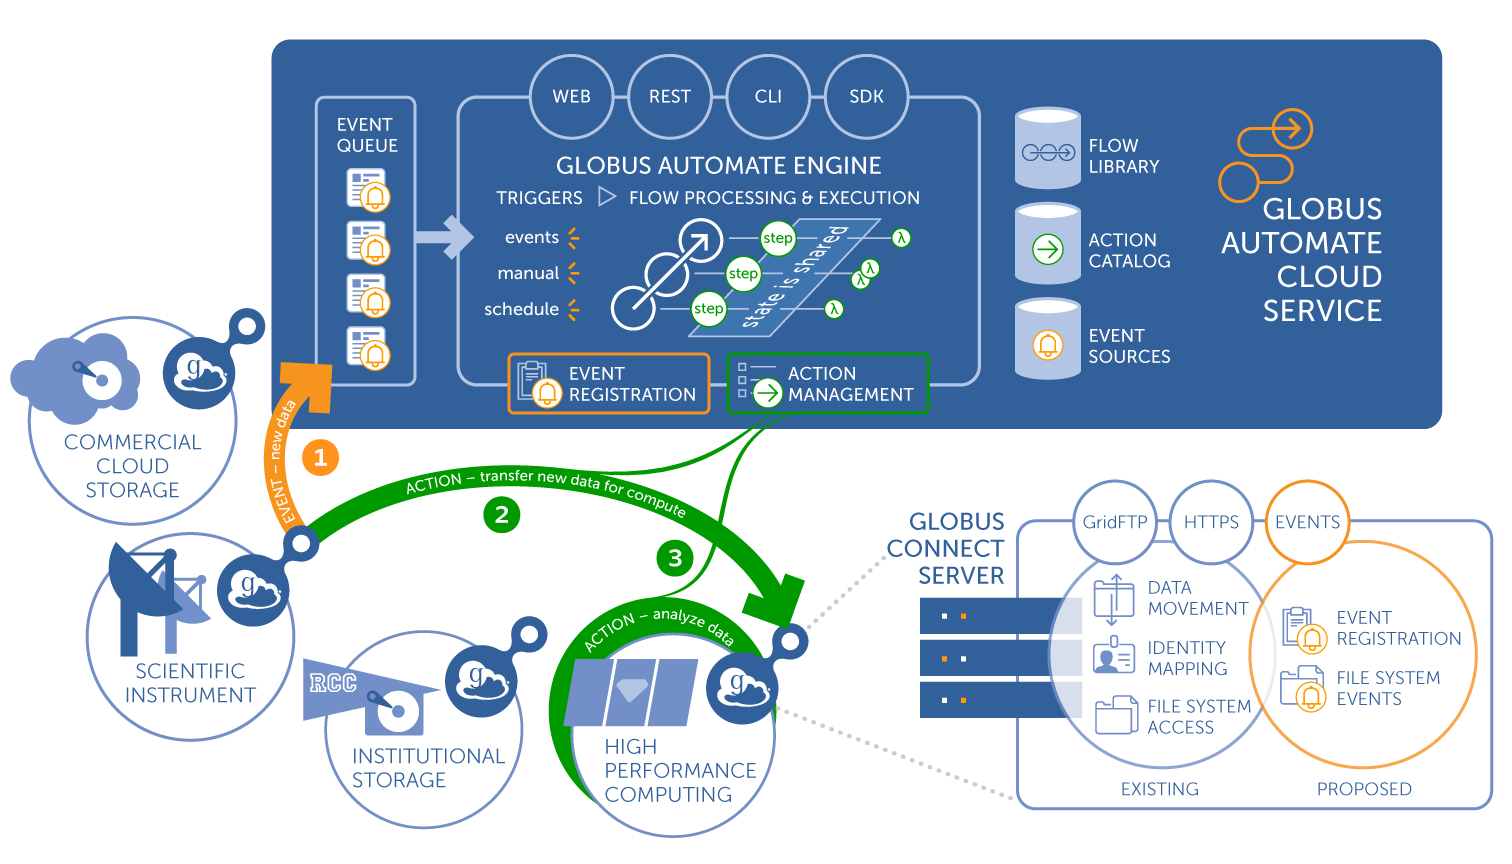
\includegraphics[width=6in]{Figs/automate.png}}
  \caption{Globus Automate architecture, showing the cloud service at top, services that it
    manages below, and the extended Globus Connect internals at bottom right. Also, a flow
    comprising 
    (1) an event (data created at instrument), (2) a transfer action, and (3) an analysis action.
\label{fig:diffuse}}
\end{figure}


\subsection{Capturing and responding to events}
Globus Automate is reliant on the ability to monitor and receive events from
external services. 
We define a \darkcode{globus\_event} REST API to be implemented by any service that wants to produce 
events for consumption by Globus Automate
and a simple queuing mechanism to reliably deliver events.
Our goal is to make it simple for a service to produce and consume events, 
while also enabling performant and robust event delivery.
The \darkcode{globus\_event}  API, 
allows for a client (e.g., Globus Automate) to register with a service (e.g., Globus Connect) 
to receive events (e.g., file created) that match event-specific criteria (e.g., all files matching 
a path expression). 
%The API includes methods such as
%the following, some taking a \bluecode{<registration\_id>} as a parameter:

%\begin{itemize}
    %\item \code{/globus\_event/v1}\darkcode{/introspect}: 
    %Returns monitorable events and event matching parameters.
    %\item \code{/globus\_event/v1}\darkcode{/register}\code{/}\bluecode{<registration\_id>}: 
    %Register to send matching events to a specified URL. This registration will be identified by
    %the \darkcode{<registration\_id>} UUID.
    %\item \code{/globus\_event/v1}\darkcode{/cancel}\code{/}\bluecode{<registration\_id>}: 
    %Stop sending events from a previous registration.
%\end{itemize}
%\vspace{1ex}

Globus Automate (or any other client)
can use the \darkcode{/introspect} method on a service 
to determine what event types are available from that service---and,
for each event type, what parameters can be use to match events. 
For example, Globus Connect endpoints could offer
events such as ``file created'' and ``file deleted,'' 
each accepting a path matching expression as a parameter,
so that Globus Automate can request notifications when 
files in a certain directory are created or deleted.
Globus Automate will \darkcode{/register} 
for events matching particular parameters, providing a URL to which the service should POST the 
events, along with a globally unique \bluecode{<registration\_id>} UUID.  In the event of a 
communication error, Globus Automate can idempotently retry the same \darkcode{/register} call, such 
that if the service already knows the \bluecode{<registration\_id>} it can respond as such.
When events are no longer needed from a service, Globus Automate will \darkcode{/cancel} the 
registration 
using the same \bluecode{<registration\_id>}.

\subsection{Invoking and managing actions}
The Globus Automate engine invokes an action in an external service to 
perform a step of an automation flow. Each external service must implement a
simple REST API for introspection, execution, and management. 
When registering an external service, the service must 
define the actions that it supports, for each with
a unique name, description, input and output parameters, 
and whether it runs synchronously (quickly, blocking)
or asynchronously (slowly, non-blocking).
The action API focuses only on the information 
needed by Globus Automate.
It may be implemented alongside any other REST API offered by a service.
%Each POST specifies a \darkcode{/method} and typically also a \bluecode{variable}:

%\begin{itemize}
    %\item \code{/globus\_automate/v1/action}\darkcode{/list}: 
    %List the actions supported by this service.
    %\item \code{/globus\_automate/v1/action/}\bluecode{<action\_name>}\darkcode{/introspect}: 
    %Return parameters that can be passed to this action, 
    %with a type and if the parameter is required/optional. 
    %\item \code{/globus\_automate/v1/action/}\bluecode{<action\_name>}\darkcode{/run}:
    %Execute the action, given a parametrized document matching
    %the schema returned from the \darkcode{/introspect} method.
    %\item \code{/globus\_automate/v1/action/}\bluecode{<action\_id>}\darkcode{/status}: 
    %Retrieve the state of the given asynchronous action instance. 
    %If the action is complete, return the output document.
    %\item \code{/globus\_automate/v1/action/}\bluecode{<action\_id>}\darkcode{/cancel}: 
    %Cancel an asynchronous action instance.
    %\item \code{/globus\_automate/v1/action/}\bluecode{<action\_id>}\darkcode{/release}: 
    %Release an action instance. 
%\end{itemize}
%
%\vspace{1ex}

The action model is simple: JSON document in, JSON document out, with a simple protocol to ensure 
reliable, once-and-only-once execution.
When Globus Automate needs to run an action as part of a flow, it calls the service's action 
\darkcode{/run} method with an input JSON document with the appropriate parameters, and a globally 
unique \code{<action\_id>}.  
If Globus Automate does not receive a response from \darkcode{/run}, for example due to a network 
error, 
it can repeat the \darkcode{/run} call with the same \code{<action\_id>}, allowing the service to 
recognize duplicate requests.  
In the case of asynchronous actions, Globus Automate will then periodically call \darkcode{/status} 
to check if the action  has completed. 
If the action has completed, \darkcode{/status} will return the output JSON document with the 
appropriate parameters.  
 
Once Globus Automate sees that an action has completed, it calls \darkcode{/release} 
so that the service can forget about the \code{<action\_id>}.  
If an action takes longer than a flow step's configured timeout,
Globus Automate may call \darkcode{/cancel}. 
If a service does not recognize the \darkcode{<action\_id>} in a \darkcode{/cancel} or 
\darkcode{/release}, 
it should assume it was previously canceled or released, and return an appropriate error. 
After some extended period (e.g., 30 days after completion),
a service can forget any \code{<action\_id>} that is not canceled or released. 

Some actions may require human interaction.  For example, as part of 
the Globus data publication platform we aim to implement 
a web-based form entry service, 
with configurable JSON schema and form configuration. 
This service will be used for such purposes 
as simple user prompts to complex metadata entry and curation.
Such services will be integrated with Globus Automate as asynchronous actions.

\subsection{The Globus Automate engine.}
Globus Automate is responsible for executing end-to-end automation flows \emph{reliably}, 
from event registration and processing for triggers to
flow (i.e., state machine) execution and action invocation. 
After review of several workflow models, such as Amazon Simple
Workflow Service~\cite{AmazonSWF}, Netflix's Conductor~\cite{conductor}, and Apache 
Airflow~\cite{airflow}, 
we choose to leverage
Amazon Step Functions (ASF)~\cite{AmazonSteps} for implementing and managing flows.
ASF is provided by AWS as a managed service for reliably 
and scalably executing state machines (i.e., automation flows);
its declarative and intuitive JSON-based state machine language allows non-experts
to define
flows and its flexible execution model allows Globus Automate
to execute arbitrary actions.

Globus Automate uses parameterized Lambda functions~\cite{AmazonLambda} to execute actions. 
When creating a flow, Globus Automate calls \darkcode{/introspect} 
to determine the input and output parameters for an action. It then creates 
parametrized Lambda functions for that action. 
For asynchronous actions multiple Lambda functions are created (i.e., start, monitor).
When a user deploys an automation flow, Globus Automate translates the user's state machine 
with user-friendly action and event names into a state machine that invokes the appropriate 
Lambda functions and manages the flow of state between actions. 
Its deployment requires that the user specify both how its execution may be triggered and the source 
of
the JSON document to be provided as input to the first step of the state machine. 
(The input JSON document may contain both static content and 
dynamic content provided by the trigger.)
% Triggers not yet supported
%A trigger may be
%\textbf{manual}: a user executes the flow through a call to the Globus Automate REST API, 
%with a JSON input document;
%\textbf{event}: i.e., triggered by receipt of a specified event from a specified service, 
%with the event as the dynamic JSON input document; or
%\textbf{schedule}: a particular start time or periodic start, with a dynamic JSON input document 
containing the time.
%The deploying user can also set permissions to indicate who
%may execute the flow, administer its deployment, and monitor or manage flow executions.

Globus Automate wraps all logic for registering and interacting with external event- and 
action-providing services.  Currently these capabilities are exposed as a REST API. 
In the future we intend to enhance the Globus web interface to make it 
easy for users to register action and event services,
and to deploy, execute, and manage automation flows.
%As not all users will be comfortable authoring JSON, 
%we will also develop a simple graphical user interface (GUI) in which users can search for and 
select
%registered events and actions, create flows from actions with retry and timeout parameters, and 
deploy flows with triggers. 
%This interface (and the underlying REST API) will also allow users to view and modify previously 
deployed flows, monitor and manage executions of their deployed flows (e.g., cancel a running flow), 
view the events
%that triggered the flow, interrogate the JSON state document at any
%point of the flow, and view the status of actions (e.g., success or failure).
%Globus Auth will provide end-to-end security.

\subsection{Automation Use Cases}

We present two use cases in which Globus Automate is currently being applied. These
use cases highlight the benefits of automation for analysis and publication activities
conducted at light sources.

\textbf{Neuroanatomy analysis:} We have applied a prototype version of Globus Automate
to support neuroanatomy experiments that rely on
X-ray microtomography at the Advanced Photon Source (APS) 32-ID beamline to
characterize the neuroanatomical structure of large (cm) unsectioned brain 
volumes~\cite{kasthuri2015saturated}, as shown in \figurename{~\ref{fig:brains}}. 
Datasets, generated at $>$20GB per minute, are processed
with a complex reconstruction pipeline 
comprising many machines, tools, and services.  
Globus Automate is used to move data from beamline to remote computers,
execute Automo~\cite{Automo} and TomoPy~\cite{gursoy2014tomopy} 
to generate preview images. Simultaneously, machine learning models
are applied (automatically) to estimate the center of rotation. This value and the resulting 
images are returned to beamline scientists to guide instrument positioning. Once the center value 
has been verified the flow continues by performing the full reconstruction. Results are moved to 
persistent storage for distribution, cataloged with
provenance metadata, and precomputed to be visualized with Neuroglancer~\cite{Neuroglancer}. 

\begin{figure*}[t!]
	\centering
	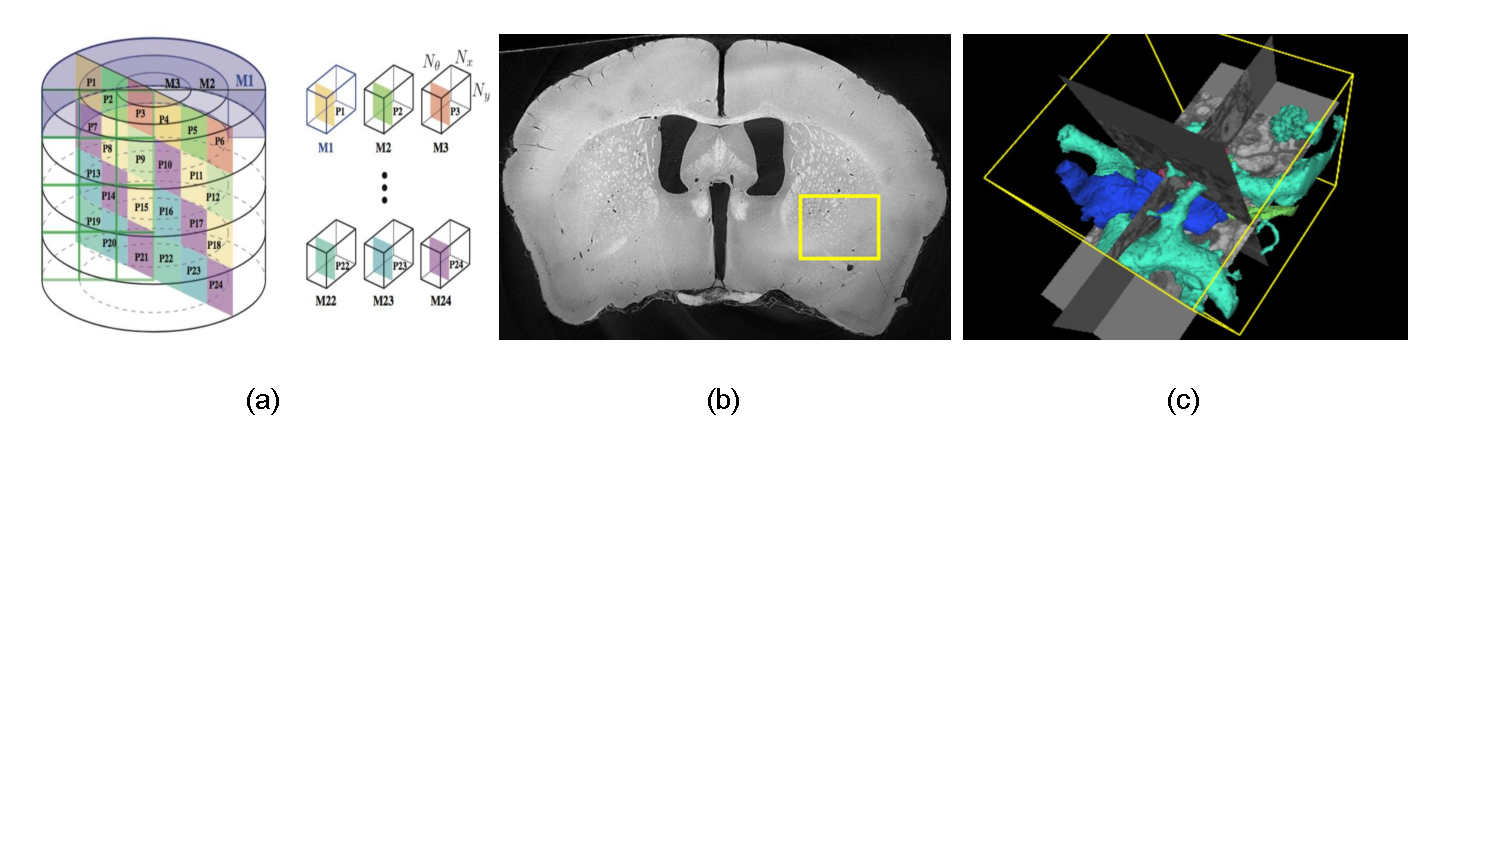
\includegraphics[trim={0.7cm 8.6cm 1.5cm 0cm},clip,width=0.99\textwidth]{Figs/brains.pdf}
	\caption{From left to right: Schematic diagram showing data acquisition process;
	coronal cross section of a reconstructed brain; and
	3D rendering of a reconstructed brain volume using Neuroglancer.}
	\label{fig:brains}
\end{figure*}


\textbf{Data publication:} We are using the prototype system to develop
flexible data publication pipelines for MDF that combine machine and human
steps. Our aim here is to provide an automated deposit mechanism in 
which users define a dataset to be published (via a reference
to a Globus endpoint) and the automation flow manages the steps required
to make that data accessible in MDF. In one example, the workflow
will transfer data to an intermediary location for processing 
and also to a permanent storage location for publication. That 
dataset will be processed with 
a community code to extract materials-specific metadata
from the dataset. This metadata will be used to register the dataset in 
in the NIST Materials Resource Registry, Citrination, or
other community registries, and also to index the dataset
in the MDF discovery index. Before the data is to be made
accessible the flow will notify MDF curators of its arrival
and wait until they have approved the dataset for publication
before progressing. A unique identifier will 
be created for the dataset, using user-defined and automatically
extracted metadata. Finally, access permissions will be 
modified such that the metadata is discoverable
and the dataset is accessible. 


\section{TRANSFORMATION, ANALYSIS, AND VISUALIZATION}

The requirement to transform and analyze results is common across light source science.
Yet, the specific analyses and cyberinfrastructure required to support analyses
are often developed by beamline scientists and are infrequently shared 
amongst researchers working in similar fields. This is clearly inefficient as it 
requires beamline scientists to obtain expertise in several unnecessary areas 
(e.g., developing cyberinfrastructure to support real-time machine learning analyses) 
and leads to significant duplication. 
As scientists increasingly look towards new machine learning approaches for various
tasks (e.g., center finding, error detection, image segmentation), 
these challenges are likely to become more significant. 
To address these challenges we are developing  
%To advance beamline science and federate access to 
%advanced computing capabilities analytical tools, generalizable solutions that can be applied 
%across domains are needed. As such, we are actively developing 
the Data and Learning Hub for Science (DLHub) which aims to 
support the deposit and sharing of machine learning models, 
on-demand inference using these models, and a high performance
computing environment for training models. 


% KC: I dont think this fits here. 
%These data can then be used with visualization tools. For example, one group using Petrel stores 
%pre-computed visualizations on the Petrel storage service and using Glbous' HTTPS support is able 
%to stream data from Petrel into a locally hosted Neuroglancer deployment. This makes data that are 
%automatically reconstructed globally accessible as 3D 
%visualizations through a simple Web interface.


\subsection{DATA AND LEARNING HUB FOR SCIENCE (DLHUB)}
 
DLHub is a service to promote, simplify, and speed the widespread adoption and
usage of machine learning and deep learning techniques by researchers in
disciplines ranging from materials science to chemistry, physics, cosmology,
and biology. The co-emergence of large amounts of available datasets, movement
towards cohesive data services, and new machine learning capabilities, creates
a unique opportunity to leverage and integrate these data streams to allow for
machine learning techniques to guide and, indeed, lead discovery efforts.
 
Thus, we are developing DLHub a self-service platform for publishing,
applying, and creating new machine learning models. DLHub
will provide: 1) publication capabilities to make models more discoverable,
citable, and reusable; 2) the ability to easily run or test existing models;
and 3) links to the data and computing infrastructure to re-train models for
new applications. Users will benefit from DLHub in many ways. Data scientists
can publish their models (i.e., architectures and weights) and methods.
Materials scientists can apply existing models to new data with ease (e.g., by
querying a prediction API for a deployed mode) and create new models with
state-of-the-art techniques. Together, these capabilities will lower barriers
to employing machine learning, making it easier for researchers to discover
and benefit from the most recent advances in machine learning.

\subsection{DLHUB ARCHITECTURE} 

DLHub is operated as a cloud-hosted service that offers a REST API to
publish, search, and invoke models. DLHub serves models and transformation
codes across remote \textit{execution sites}.  The REST API is secured with
Globus Auth \cite{tuecke2016globus} and offers endpoints for publishing, searching, and invoking
models. We provide a Python SDK to simplify use of the service. In future
work, we aim to develop a user interface for many of these tasks.  We have defined a
simple metadata schema for describing models.  Users who wish to deposit a
model must provide this metadata and a container with their trained model.
 
When invoking a model, users must first select the specific model to use
(discovered via searching the list of published models) and provide a set of
data to be passed to the model. At present, all input data is described in
JSON.  DLHub then executes the model for each item in the input JSON and
returns JSON-based results to the user.

DLHub relies on the Kubernetes container orchestration system to manage the
deployment of containerized codes and models on an execution site.  Models and
transformation logic are wrapped in Docker containers for three primary
reasons:  1) to standardize their execution interface, regardless of
implementation or language; 2) to enable the encapsulation of their vastly
different software requirements; and 3) to allow them to be scaled by deploying multiple instances of the containers. In DLHub, a containerized model is referred to as a \textit{servable}.  When a code is
published in DLHub, it is automatically packaged with a custom DLHub Python
library to provide a standard execution interface to facilitate remote
invocation. DLHub Servables can be deployed at execution sites and invoked
directly through DLHub.  A single servable may serve results for many
inference jobs and the same servable may be deployed several times to meet
user demand.

Each execution site is connected to the DLHub service through ZeroMQ (ZMQ)
channels, providing a high-performance and reliable mechanism to transmit
jobs. We use the Parsl parallel scripting library~\cite{parsl} to manage the
execution infrastructure by deploying and managing servables. Each site
includes a Parsl \textit{foreman} and a ZMQ receiver.  The ZMQ receiver is
used to receive inference jobs from the DLHub service.  The Parsl foreman is
then responsible for taking these inference jobs and executing them on one or
more servables. This task includes submitting work to existing servables or
deploying new ones if  one is not available. Parsl uses IPyParallel and a
pilot job  model to perform remote execution within a container.  Each
container is deployed with an \textit{ipengine} that  connects back to the
Parsl foreman to receive jobs.  This two-tier design enables multi-level
caching, with both Parsl and cloud-hosted caches enhancing response time.
Requests can also be  batched at the cloud level before being transmitted to
execution sites to improve throughput. While the primary mode for execution is
via the DLHub service,  for low latency jobs we also allow users to establish
a direct connection to the execution site. This model allows for DLHub to be
easily integrated in light source workflows by streaming data from the
acquisition machine to DLHub for transformation or inference.

\subsection{DLHub USE CASES}
We present two separate uses cases of the DLHub service each highlighting
key capabilities. DLHub analysis pipelines were created for these
use cases to simplify invocation on PetrelKube and within Amazon Web Services.

\textbf{Prediction of Metallic Glass Forming Compositions.}
Metallic glasses are an important class of materials that promise
improved durability, corrosion resistance, and mechanical behavior in harsh
environments. However, discovery of metallic glass forming materials is
particularly challenging due to the lack of theories that can predict which
alloys can be formed into metallic glasses. Ren \emph{et al.}
trained a machine learning model to predict glass-forming ability using data 
from the materials literature, and used it to identify new Co-V-Zr metallic glasses
via high-throughput experiments at Stanford Linear Accelerator
Laboratory (SLAC). By adding the SLAC data to the training set of the model,
they found its accuracy improved for many other types of alloys.

The associated machine learning model was contributed to DLHub as a
serialized scikit-learn Random Forest model. Containers were prepared to serve the
model, which take a list of elments as inputs return the predicted glass-forming ability
for that alloy system. An example Jupyter notebook was then prepared to use the model in DLHub 
to generate ternary plots showing areas of highest metallic glass forming likelihood \ref{fig:dlhub-glass}.

\begin{figure}[h]
  \centerline{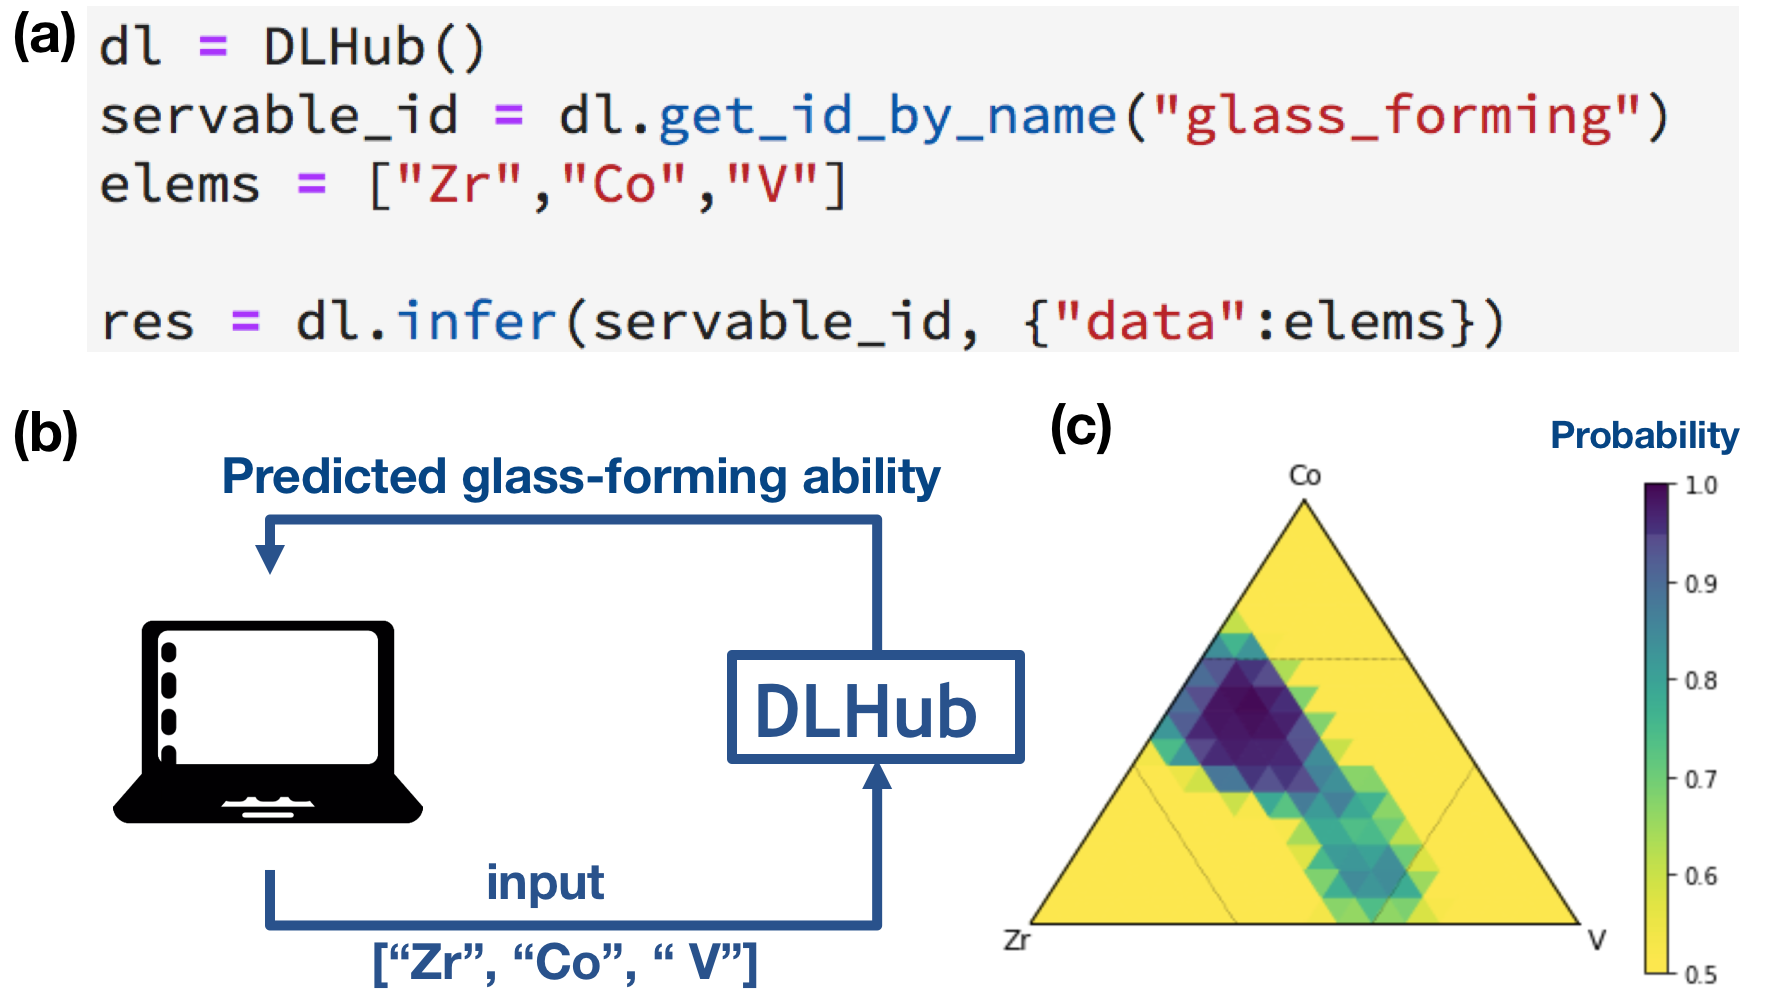
\includegraphics[width=5in]{Figs/DLHub-metallic-glass.png}}
  \caption{Predicting metallic glass forming ability with DLHub. (a) Example code showing instantiation of DLHub Python client, selection of model, and inference against that model. (b) A user submits a set of three elements and sends to DLHub service for prediction. User receives the predicted glass-forming ability as an output. (c) Displaying the results of the model for Zr, Co, V inputs as a ternary diagram.
\label{fig:dlhub-glass}}
\end{figure}

\textbf{Batch Classification of Beamline X-Ray Scattering Data.}
Classifying streaming data or archived data from beamlines at national user
facilities promises to aide future data discovery, promote data reuse, speed
analyses, and to allow users to receive near real-time feedback on the state
of their experiments. For example, if a model is able to automatically
determine that a beam is misaligned, an experimental session may be saved from
waste by user intervention.

The classification model here enables the multi-label classification of X-Ray
scattering data with 17 potential labels (e.g., ``beam off image", ``FCC",
``BCC", ``polycrystalline", ``high background", ``strong scattering") \cite{wang2017x}. The
classification model is a Tensorflow 1.4 implementation in Python 2.7 of a
convolutional neural network following the ResNet architecture. Original
training data comprised simulated data and experimental data tagged by experts
collected at National Synchrotron Light Source (NSLS) at Brookhaven National
Laboratory as described in Wang et al. This pretrained model and dataset was
contributed to DLHub by Wang and Yager et al. and the original source code has
been made available to the public on Github\cite{wang2017xcode}. Containers were created to serve
the model and handle data transformation from input image files to the
required input: 256x256 numpy arrays.

\begin{figure}[h]
  \centerline{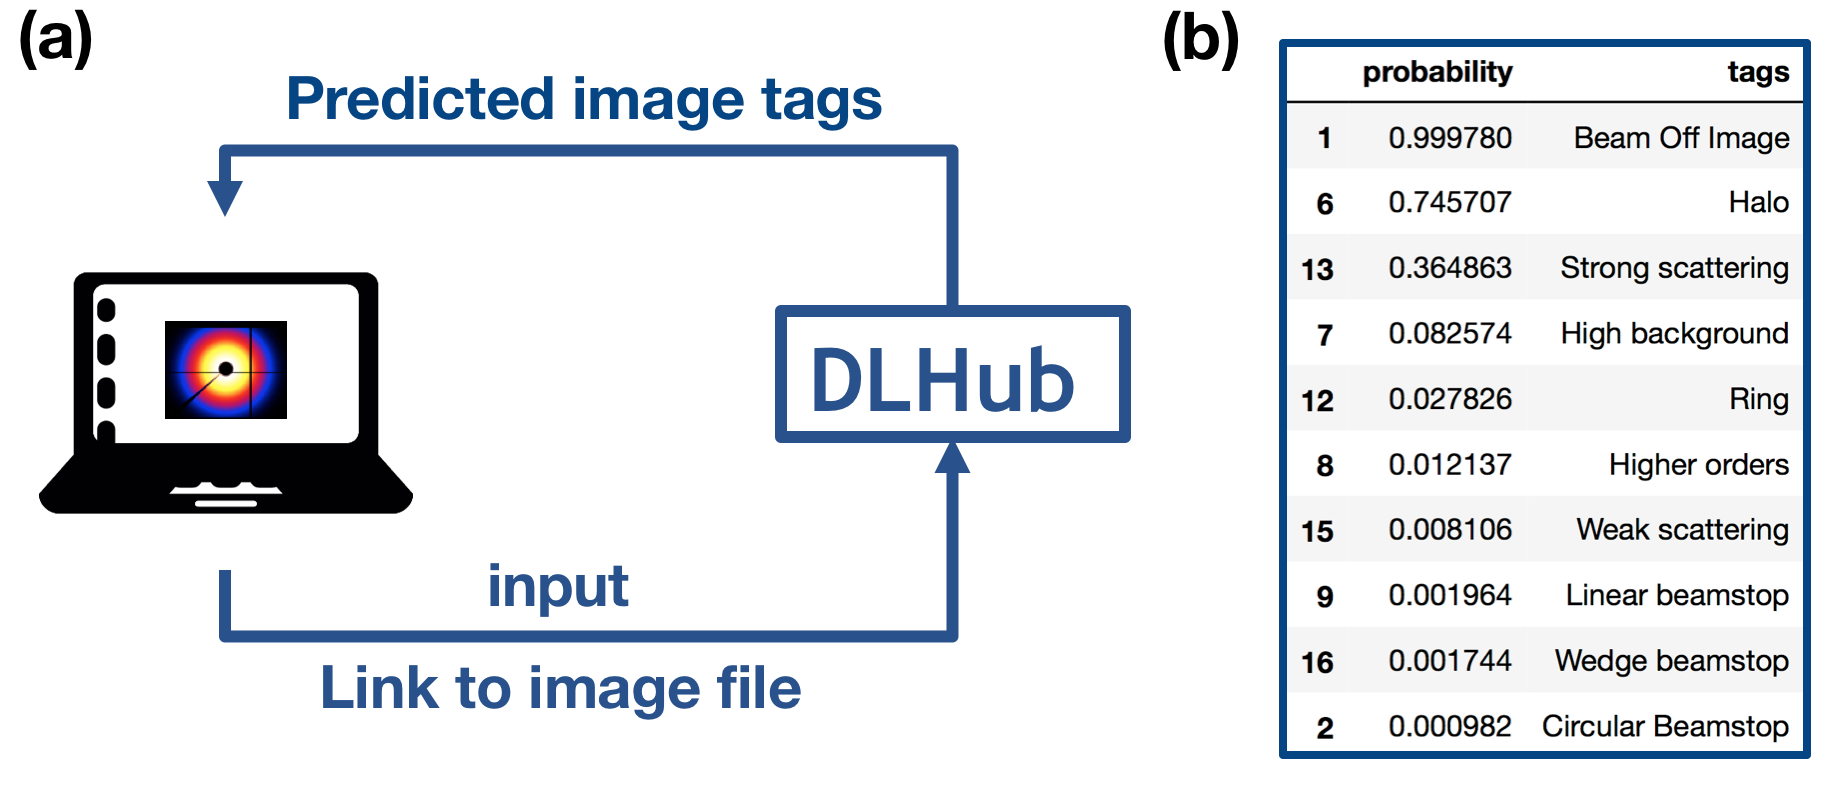
\includegraphics[width=5in]{Figs/DLHub-BNL.png}}
  \caption{Tagging X-Ray scattering images with DLHub. (a) User sends pointers to X-Ray scattering images to the DLHub service. (b) DLHub returns a list of most likely tags for the image.
\label{fig:dlhub-bnl}}
\end{figure}
\section{RELATED WORK}

\ryan{Might need something about outsourcing.}

The requirement for automation in science has been well studied
studied~\cite{king2009automation, deslippe2014workflow, chard17ripple} and 
as such there are many automation systems currently in use. Coles et 
al.~\cite{coles2005ecses,coles2006science} developed an automated small molecule crystallography 
service that manages the end-to-end-flow from sample receipt to results dissemination. 
The SPOT framework~\cite{deslippe2014workflow} powers similar pipelines for Berkeley's Advanced 
Light Source. Scientific workflow engines, such as Galaxy~\cite{galaxy}, Parsl~\cite{parsl}, 
Pegasus~\cite{pegasus}, Swift~\cite{wilde2011swift}, and Taverna~\cite{taverna},
enable the fault-tolerant and reproducible execution of pipelines comprising various tools and 
services. While some, such as Teverna, support Web service composition, these tools are generally 
designed to facilitate dataflow modeling and the execution of sequences of tools. This is in 
contrast to Automate, which aims to orchestrate a mix of custom software and human-in-the-loop 
tasks.

\ian{PNNL work~\cite{thomas2015towards}. Helmholtz work~\cite{gehrke2015high}.}
% BNL work~\cite{deslippe2014workflow} (SPOT).

The need to reliably catalog and publish data has led to the development of several 
tools~\cite{chard15publication,wilkinson16,costello09pub}. Indeed, many of these platforms are 
widely in use (e.g., Dataverse~\cite{dataverse}, DuraCloud~\cite{duracloud}, and 
figshare~\cite{figshare}).
Our approach 
with the MDF is to provide a generalizable platform to accommodate diverse communities, datasets, 
and publication scenarios by outsourcing the tools required to mint identifiers, catalog metadata, 
and search over distributed datasets to specialized services.

\ian{Reference ModelHub~\cite{miao2017towards}. Velox for rapid model 
serving~\cite{crankshaw2014missing}. and~\cite{kumar2017data}}
% Velox: https://blog.acolyer.org/2015/02/02/the-missing-piece-in-complex-analytics/

\ryan{DLHub RW?}

As machine learning becomes 
increasingly pervasive there is a growing requirement for services to publish, share, and serve 
models. High performance, low latency 
model serving is necessary to facilitate the integration of machine learning solutions into 
everyday tasks. To this end, various model serving platforms have been 
developed~\cite{clipper, crankshaw2014missing, tfserving, awssagemaker}. Clipper~\cite{clipper} and 
Tensorflow Serving~\cite{tfserving} use RPC-based invocations solutions to minimize the overhead 
when invoking models, providing extremely low latency serving solutions. In addition, Tensorflow 
serving facilitates extreme-scale deployment of models, enabling integration in large-scale 
platforms, such as shopping carts. One limitation of these systems is their strict enforcement of 
the types of models and transformation logic that can be served. For example, Tensorflow Serving 
restrict servable types to be those that can be exported as Tensorflow graphs and provides minimal 
support for transformation codes.

\ryan{I haven't read the modelhub paper -- not entirely sure this usage is accurate}
Similarly, model publication services, such as Kipoi~\cite{kipoi} and 
ModelHub~\cite{miao2017towards}, have been established to publish models along with their trained 
weights and metadata describing their inputs and outputs, graph design, training and 
validation datasets, accuracy, as well as information relating to citation and authorship. Such 
tools are necessary to disseminate machine learning models and make them available to the 
community.

DLHub differs from these solutions by combining publishing capabilities, model serving 
functionality, and the resources required to train and invoke models on-demand. DLHub is designed 
to accommodate arbitrary models and servables through containerization, removing the restrictions 
of serving systems such as Tensorflow Serving. Leveraging descriptive metadata, inspired by 
Kipoi~\cite{kipoi}, and the Globus Search service, DLHub enables the publication of models such 
that users can search and find models, retrain them on specific datasets, and invoke them against 
data on-demand. 

% \ryan{We really need to write a paper surveying model serving platforms.}

\section{SUMMARY}









\section{ACKNOWLEDGMENTS}

This work was supported in part by DOE contract DE-AC02-06CH11357 and by award 70NANB14H012 from the U.S.\  Department of Commerce, National Institute of Standards and Technology as part of the Center for Hierarchical Materials Design (CHiMaD).
We are grateful to colleagues at the Argonne Photon Source and other synchrotron light sources
for many helpful discussions.

% References

\nocite{*}
\bibliographystyle{aipnum-cp}%
\bibliography{Bibs/refs}%


\end{document}
